\documentclass[12pt]{article}

\usepackage{hyperref}
\usepackage[utf8]{inputenc}
\usepackage{graphicx}
\usepackage[xindy, acronym ,toc]{glossaries}

\graphicspath{ {images/} }

\title{Artificial Intelligence}
\author{
        Henry Huck \\
        Master Specialisé - HEC \\
        \and
        Romain Lapeyre\\to
        Grande Ecole - HEC\\
}
\date{\today}

\makeglossaries
\makeindex

%%%%%%%%%%%%%%%%%%%%%%%%%%%%%%%%%%%%%%%%%%%%%%%%%%%%%%%%%%%%%%%%%%%%%%%%%%%%%%%%
%%%%%%%%%%%%%%%%%%%%%%%%%%%%% Glossary Definitions %%%%%%%%%%%%%%%%%%%%%%%%%%%%%
%%%%%%%%%%%%%%%%%%%%%%%%%%%%%%%%%%%%%%%%%%%%%%%%%%%%%%%%%%%%%%%%%%%%%%%%%%%%%%%%

\newacronym{NLP}{NLP}{Natural Language Processing}
\newacronym{AGI}{AGI}{Artificial General Intelligence}
\newacronym{ASI}{ASI}{Artificial Super Intelligence}
\newacronym{ANI}{ANI}{Artificial Narrow Intelligence}

\newglossaryentry{neuralLabel}
{
  name={Neural Network},
  description={}
}

\newglossaryentry{petaflops}
{
  name={petaFLOPS},
  description={One petaflop is $10^15$ floating operations per second}
}

%%%%%%%%%%%%%%%%%%%%%%%%%%%%%%%%%%%%%%%%%%%%%%%%%%%%%%%%%%%%%%%%%%%%%%%%%%%%%%%%
%%%%%%%%%%%%%%%%%%%%%%%%%%%%%%%%%%%% Title Page %%%%%%%%%%%%%%%%%%%%%%%%%%%%%%%%
%%%%%%%%%%%%%%%%%%%%%%%%%%%%%%%%%%%%%%%%%%%%%%%%%%%%%%%%%%%%%%%%%%%%%%%%%%%%%%%%

\begin{document}

\maketitle
\thispagestyle{empty}
\pagenumbering{gobble}

\pagebreak

%%%%%%%%%%%%%%%%%%%%%%%%%%%%%%%%%%%%%%%%%%%%%%%%%%%%%%%%%%%%%%%%%%%%%%%%%%%%%%%%
%%%%%%%%%%%%%%%%%%%%%%%%%%%%%%%%%%%% Quote Page %%%%%%%%%%%%%%%%%%%%%%%%%%%%%%%%
%%%%%%%%%%%%%%%%%%%%%%%%%%%%%%%%%%%%%%%%%%%%%%%%%%%%%%%%%%%%%%%%%%%%%%%%%%%%%%%%

\phantom{TEXT}
\thispagestyle{empty}
\pagenumbering{arabic}

\vspace{200pt}
\begin{quotation}
\noindent \textbf{Human:}  \textit{\lq What is the purpose of emotions ?\rq }
\\

\noindent \textbf{Machine:} \textit{\lq I don't know.\rq}
\end{quotation}

\vspace{200pt}

\begin{flushright}
   From Google's research paper \lq A Neural Conversation Model\rq. \cite{seq2seq}
\end{flushright}


\pagebreak

%%%%%%%%%%%%%%%%%%%%%%%%%%%%%%%%%%%%%%%%%%%%%%%%%%%%%%%%%%%%%%%%%%%%%%%%%%%%%%%%
%%%%%%%%%%%%%%%%%%%%%%%%%%%%%%% Table of contents %%%%%%%%%%%%%%%%%%%%%%%%%%%%%%
%%%%%%%%%%%%%%%%%%%%%%%%%%%%%%%%%%%%%%%%%%%%%%%%%%%%%%%%%%%%%%%%%%%%%%%%%%%%%%%%

\smallskip

\tableofcontents

\pagebreak

%%%%%%%%%%%%%%%%%%%%%%%%%%%%%%%%%%%%%%%%%%%%%%%%%%%%%%%%%%%%%%%%%%%%%%%%%%%%%%%%
%%%%%%%%%%%%%%%%%%%%%%%%%%%%%%% Acknowledgements %%%%%%%%%%%%%%%%%%%%%%%%%%%%%%%
%%%%%%%%%%%%%%%%%%%%%%%%%%%%%%%%%%%%%%%%%%%%%%%%%%%%%%%%%%%%%%%%%%%%%%%%%%%%%%%%

\section*{Acknowledgments}
\addcontentsline{toc}{section}{Acknowledgments}

\pagebreak

%%%%%%%%%%%%%%%%%%%%%%%%%%%%%%%%%%%%%%%%%%%%%%%%%%%%%%%%%%%%%%%%%%%%%%%%%%%%%%%%
%%%%%%%%%%%%%%%%%%%%%%%%%%%%%%% Intro %%%%%%%%%%%%%%%%%%%%%%%%%%%%%%%%%%%%%%%%%%
%%%%%%%%%%%%%%%%%%%%%%%%%%%%%%%%%%%%%%%%%%%%%%%%%%%%%%%%%%%%%%%%%%%%%%%%%%%%%%%%


\section*{Introduction}\label{introduction}
\addcontentsline{toc}{section}{Introduction}

\smallskip

{\em \lq Can machines think ?\rq }. This is the question Alan Turing raised in
his paper {\em The Imitation Game} \cite{Turing}. In order to answer this
question, Turing designed a test, a Game, that a {\em thinking} machine would be
able to pass. Very simply, a machine would pass this test, if a human
interrogator giving written questions to subjects in two different rooms, one
subject being a machine, and the other one being a human, would not be able to
tell in which room the machine is by examining its answers. \\

An AI simulating a 13 years old Ukrainian boy is said to have pass this famous
test \footnote{\href{http://www.bbc.com/news/technology-27762088} {BBC - Eugene
Goostman}}. However, this result was highly controversial due to the setting of
the test (short Q\&A sessions), and the deceptive strategy adopted in order to
pass the test. (i.e. pretending to be a child). According to those critics,
we're still far from creating an Artificial Intelligence that could perform as
well as a Human in every domain, and not only in \gls{NLP}. We'll call such an
AI an \gls{AGI}, as it has the same intelligence as a human. \\

But, are we really far from building human like AI ? In his book {\em The
Singularity is near} \cite{Kurzweil}, futurist Ray Kurzweil bases his theory
upon the fact that technological progress follows the Moore's Law
\footnote{\href{https://en.wikipedia.org/wiki/Moore\%27s_law} {Wikipedia -
Moore's Law} }, and as such, is exponential. According to him, we're accustomed
to think linearly, and subsequently not able to handle exponential progress.
Kurzweil explains that the rise of an \gls{AGI} is inevitable, and those saying
the contrary are just not thinking exponentially. Moreover, the rise of an
\gls{AGI} means that we'll have created a machine with the same level of
intelligence as a standard Human, but with a much greater computational power.
If the machine is capable of self improvement, it won't be long before it
evolves into an \gls{ASI}, an artificial intelligence with capacities so great,
that it is impossible to predict what could happen. This explosion of
intelligence is called a technological singularity. Irvin Good, a mathematician
who worked with Turing was one of the first to write about it: \\

\smallskip

\begin{quotation}
   Let an ultra-intelligent machine be defined as a machine that can far surpass
   all the intellectual activities of any man however clever. Since the design
   of machines is one of these intellectual activities, an ultra-intelligent
   machine could design even better machines; there would then unquestionably be
   an \lq intelligence explosion\rq , and the intelligence of man would be left
   far behind. Thus the first ultraIntelligent machine is the last invention
   that man need ever make \cite{Good}.
\end{quotation}

However, these theories are highly controversial, and scientists strongly
disagree on those issues. Even Turing's test is disputed. John Searle challenged
it in a thought experiment known as the Chinese Room \cite{ChineseRoom}. If an
english speaking person was put in a room, with very precise instruction (i.e. a
programm) in English, to translate a set of characters (chinese questions) into
another set of characters (the answers to those questions), so that Chinese
observers would be convinced to speak with a Chinese person, would that mean
that the person in the room {\em actually} speaks Chinese? Or would he just
simulate the ability to understand it ? For Searle, the latter is true, and a
machine who would pass the Turing Test could not be considered a {\em thinking}
machine. \\

When IBM's computer, Watson, won at the Question \& Answer game Jeopardy, Searle
called Watson \textit{\lq  An ingenous program, not a computer that can
think\rq} \footnote{
\href{http://cacm.acm.org/magazines/2012/1/144824-artificial-intelligence-past-and-future/fulltext}
{Artificial Intelligence: Past and Future}}. Nevertheless, IBM's computer Watson
{\em did} manage to win at Jeopardy!, and to beat the best players in the world.
The argument that Watson is not thinking, because it was not able to know and
realize it has won is true. However, the technical feat is here. Watson is
definitely not an Artificial General Intelligence, but it is a spectacular
example of Artificial Narrow Intelligence. \\

So even if we're not yet close to building an \gls{AGI}, we've managed to build
great \gls{ANI}s in various domains. Watson and Deep blue were good examples.
Another astonishing one is an AI developed at Google that learns to play video
Games \cite{Atari}. The team behind it used a mix of two methods, deep learning
and reinforcement learning, and the resulting AI was able to learn to play on
old Atari Games. It only used the video signal inputs, the final score and the
possible actions, \lq just as a human player would\rq. It managed pretty well on
games where reaction prevails, just like in Break Out
\footnote{\href{https://www.youtube.com/watch?v=cjpEIotvwFY} {Here is a video
demonstrating this}}, but failed to achieve similar succes where planning is
necessary. This example shows how it is possible to interact in an adaptive
maner with more complex environnments where the input is a video. \\

Speaking of more complex environment, another example of very good \gls{ANI} is
the self driving car. It is much better than human at driving, and it can do it
non-stop and in a safely way. The google car has now driven over 1 million
miles, and has been involved in only 14 accidents. The car was even not
responsible in those accidents, or was being manually driven by a google
employee. Self driving cars are to become a reality, and is a perfect example of
\gls{ANI}. \\

Right now, Artificial Intelligence may not be able to {\em think}, but several
ANIs already excel in specific areas. This means there are opportunities to
disrupt existing industries. One field of AI we deemed particularly interesting
is the Natural Language Processing. The aim of NLP is to teach human language to
machines, and make them able to understand queries formulated with natural
language. This is an important aspect of AI in order to pass the Turing test we
discussed earlier. \\

The purpose of this paper is to give a general overview of the recent
improvements in Artificial Intelligence studies. It is not intended to be a
highly technical paper, and the reader should only have minimal notions about
computer science and mathematics to understand what is being discussed.
Nonetheless, we'll provide an overview of the state of the art techniques in
Artificial Intelligence and Machine Learning, and what is being made possible
thanks to those. Thanks to this knowledge, we'll be able to discuss various
disruptive business ideas, and the impact of AI on the entrepreneurial
ecosystem. \\

Firstly, we will present a brief history of Artificial Intelligence studies, from
Turing original paper on artificial intelligence, (though the term was coined
later), to the latest models used in Natural Language Processing and their
applications.

\noindent Then, we'll examine the implications of Artificial Intelligence
progress for the Entrepreneurial Ecosystem, and the businesses that could benefit
from the latest strides. In particular, we'll see the impact on the car
industry, and the impact it may have on interfaces and the way we interact with
machines thanks to the progresses made in Natural Language Processing.

\noindent Lastly, we'll see what are today's limitations, and what remains to be
achieved before all these breakthroughs start being fully usable. We'll question
the possible rise of an Artificial Super Intelligence, and what are the caveats
expressed by some members of the scientific community.

\pagebreak

%%%%%%%%%%%%%%%%%%%%%%%%%%%%%%%%%%%%%%%%%%%%%%%%%%%%%%%%%%%%%%%%%%%%%%%%%%%%%%%%
%%%%%%%%%%%%%%%%%%%%%%%%%%%%%%% First part %%%%%%%%%%%%%%%%%%%%%%%%%%%%%%%%%%%%%
%%%%%%%%%%%%%%%%%%%%%%%%%%%%%%%%%%%%%%%%%%%%%%%%%%%%%%%%%%%%%%%%%%%%%%%%%%%%%%%%

\section{Recent improvements in ML technologies}

Artificial Intelligence has made tremendous progress over the last few years.
Compared to other disciplines, it is still relatively young, and there is still
plenty of things to be discovered. We'll present a brief history of Artificial
Intelligence studies, along with some basics concepts and results that will
allow us to understand the models discussed after. We'll then see how access to
faster computer and to Big Datasets has allowed some progress in Artificial
Intelligence.

\subsection{A bit of History}

\smallskip

Before designing his famous test, Turing laid the ground of modern computer
science, proving that every mathematical computation that could be represented
with an algorithm was possible thanks to an hypothetical machine, manipulating
a tape with zeros and ones. Now called Turing Machines, they are the ancestor
of modern computers.\cite{Turing1936}

Results in neurology research showing that the brain was a vast networks of
neurons, sending discrete electrical signal, inspired the idea of artificial
neural neurons. In 1951 Minsky and Edmonds built the SNARC, the first neural net
machine with a hardware relying on vacuum tubes.

The discipline of Artificial intelligence itself was founded later, during the
summer of 1956. It was organized by Minsky and McCarthy, and two senior
scientists of IBM. It was held at Dartmouth College, and the scientists
attending the project were to become major authors and influencers for the
decades to come. \cite{DartMouth}\\

The early programs created by the newborn field of AI used what is essentially a
tree exploration program. For a maze exploration, or a proof of a theorem, the
algorithm is simply moving forward the possibilities trying to reach a goal (the
exit of the maze, or the conclusion of the theorem). The programm is turning
back when it reaches a dead end, or can abandon a whole path and the
possibilites behind it if it is deemed unpromising. It proved successful on a
number of simple problems, where the number of possibilities, or search space,
is limited. But on larger problems, the search space would simply explode making
it impossible to explore. The idea was then to estimate sub-goals thanks to
heuristics functions specific to each problem.

\begin{figure}[ht]
    \centering
    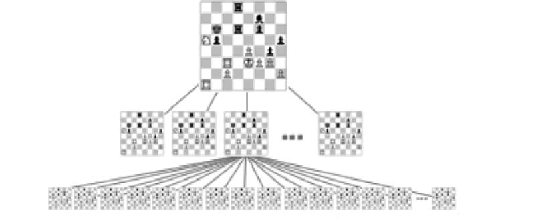
\includegraphics[width=\textwidth]{chess-tree}
    \caption{A chess exploration tree}
    \label{fig:chess_tree}
\end{figure}

\smallskip

They also focused on solving \gls{NLP}. Joseph Weizenbaum designed ELIZA, a
program giving simple canned phrases as answers. The chatterbot worked thanks to
simple  pattern matching and keyword substitution, but the result was of great
effect on some users.

Scientists were extremely confident at the time in the success of their research.
H.A. Simon declared in 1958, that \lq within ten years, a computer would be the
world's chess champion.\rq IBM's Deep Blue computer defeated Garry Kasparov only,
in 1997. They failed to properly estimate the difficulty of the problems they were
facing for many reasons.

They focused on studying logical problems, or theorem proving, problems considered
difficult for a human mind. Thus, they considered that {\em simple} tasks such as
vision would be easy to reverse engineer once more high-level problems had been
solved. This is known as the Moravec's paradox:

\begin{quotation}
  Encoded in the large, highly evolved sensory and motor portions of the human
  brain is a billion years of experience about the nature of the world and how
  to survive in it. The deliberate process we call reasoning is, I believe, the
  thinnest veneer of human thought, effective only because it is supported by
  this much older and much more powerful, though usually unconscious,
  sensorimotor knowledge. We are all prodigious olympians in perceptual and
  motor areas, so good that we make the difficult look easy. Abstract thought,
  though, is a new trick, perhaps less than 100 thousand years old. We have not
  yet mastered it. It is not all that intrinsically difficult; it just seems so
  when we do it. \cite{Moravec}
\end{quotation}

The lack of hardware resource and computational power was also one of the reason
they could not deliver what they had promised. Their examples worked on simple
cases but did not achieve significant results on more complex, real-world
applications.\\

%TODO: rephrase the introduction of paragraph
During the same period, work continued on neural nets and their possible
applications The Perceptron algorithm, created in 1957 by Frank Rosenblatt, was
a promising linear classifier. However 1969 Minsky and Papert published {\em
Perceptrons}, criticizing the possibilities offered by Perceptrons, and stating
that a single artificial neuron was not able to implement a certain logical
function, the exclusive-or function. This would have grandly limited the mathematical
possibilities of the structure, but it turned out it is actually possible. However
this result, combined with the disillusion of AI research, led to was is known as
the first AI Winter.

The generous funding of the first years were cut, and AI researched focused on
symbolic and logic programming rather than neural networks and machine learning.
In the UK, the lighthill report, evaluating the state of AI in the country,
criticized what had been accomplished, and led to a major collapse in AI
research.

AI research was now forced to focus on specific projects, and achieve results on
clear objectives. Expert Systems were one of the success of AI. It focused on
specific fields of knowledge, associating databases with logical rules
infered from experts in those fields. It helped AI revive in the 80's, as expert
systems  helped large corporation in saving millions of dollars.\\

The domain of neural network was also revived by the discovery of the back
propagation algorithm, a technique used to train neural networks. Neural
networks would start to provide commercial success in the 90's, when they
started to be  applied to character recognition and speech recognition.

Money returned to finance AI research, with several large projects, the most
emblematic being the fifth Generation Computer project, a Japanese 10 years
project aiming at revolutionizing AI thanks to super computer and highly
parallelized computations. The expectations were so high the program was doomed
to failure.

The second AI Winter came during the early 90's with the fall of expert system
and  specialized hardware. Once again, excitations was built around first
results, and  disappointment followed. However, progresses made during this
period were real,  and laid the basis for modern AI.\\

A lot of techniques and research developed in the AI field actually filtered
into  other industries, and became widespread. In fact, those applications that
have become  mainstream stopped being called AI. It is part of the AI effect,
that states that \lq When we know how a machine does something {\em
intelligent}, it ceases to be regarded as intelligent.\rq
\footnote{\href{http://www.washingtontimes.com/news/2006/apr/13/20060413-105217-7645r/}
{Fred Reed}}

%TODO: add some stuff about recent results

\pagebreak

\subsection{Why is AI progressing faster and faster?}

One of the major reason of AI first disappointments was the lack of hardware
powerful  enough to crack on the problems they were facing. Today's progress
have made hardware powerful enough to solve certain problem or achieve
significant results. How is this, and the  access to large training datasets
helping artificial intelligence ?

\subsubsection{Hardware progress}

Kurzweil's theory about the singularity may be controverted, he's right about
something: We do witness exponential progress in terms of computing power. This
is known as the Moore's Law. It states that the number of transistor on dense
integrated circuits double every two years. Hence, it can be approximately said
that the computational power available at a given price double every two years.

\begin{figure}[ht]
    \centering
    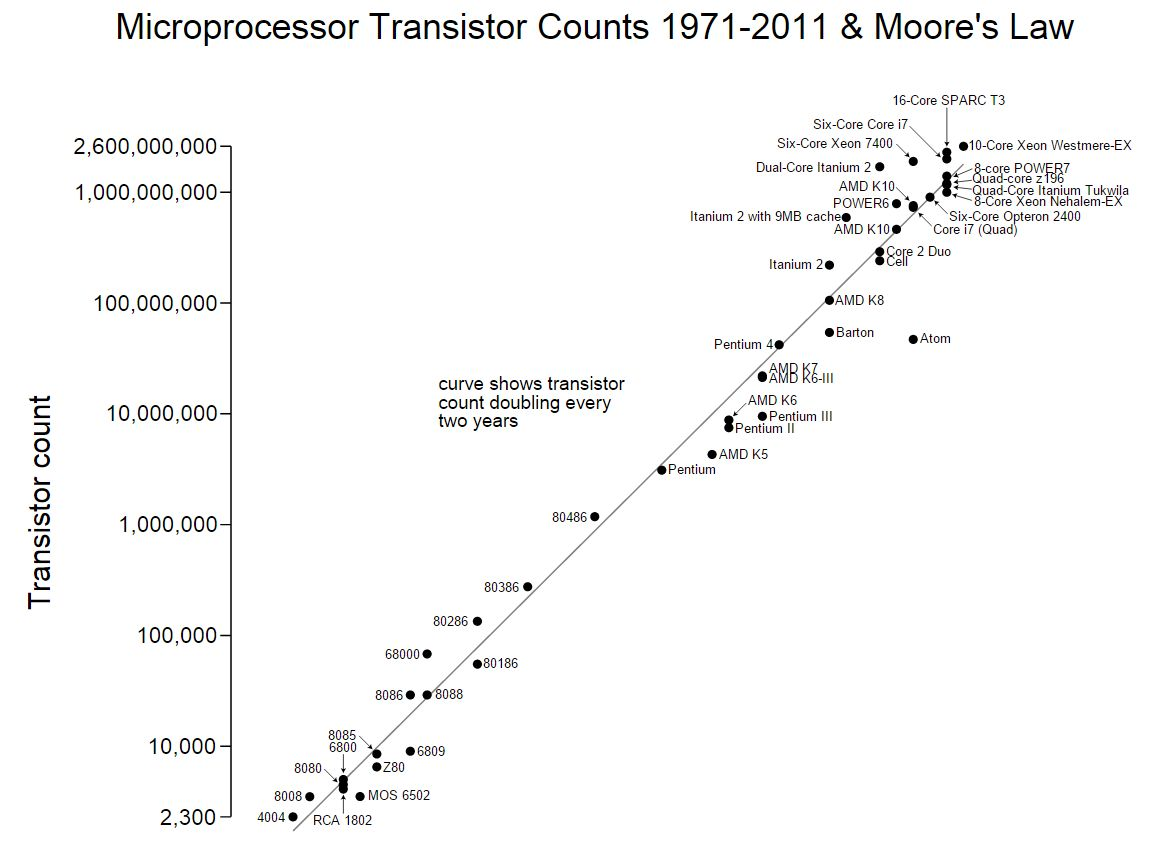
\includegraphics[width=\textwidth]{moore}
    \caption{Moore's Law}
    \label{fig:moore}
\end{figure}


We're getting access to better and better hardware, but where do we stand
compared to a human brain ? This is a bit of an apple and orange comparison, so
this is just to give an idea of what has been achieved. The world's fastest
supercomputer is Tianhe-2, in Guangzhou. It has a speed of 33.86 \gls{petaflops}
and cost about \$390 millions. During summer 2013, the largest neural network
simulation was run on a super computer a bit less powerful, on the K computer,
with a speed of about 10 petaflops.\footnote{\href{http://www.sciencedaily.com/releases/2013/08/130802080237.htm}
{Largest neuronal network simulation to date achieved using Japanese
supercomputer}} The simulation represented about 1\% of the brain, and was able
to simulate the brain activity during one second. This does not give us the
processing speed of a human brain, and does not allow to compare directly the
brain to those computer in term of raw power, but we can extrapolate, and
estimate that we would need a super computer with a speed in the exaflops, which
is $10^{18}$ flops. According to the Moore's Law, this {\em should} happen around
2020.\\

\begin{figure}[ht]
    \centering
    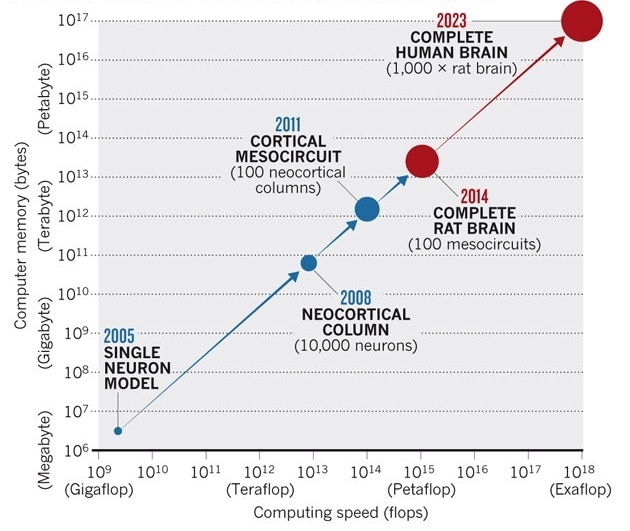
\includegraphics[width=\textwidth]{fartogo}
    \caption{When will super computer be equivalent to human brain ?}
    \label{fig:fartogo}
\end{figure}

%% moved later
%% power. The Tianhe-2 uses $24MW$ with its cooling system. The brain uses 20 W.

One other promising lead is the parallelization of computing. Thanks to more and
more performant GPUs\footnote{Too make it simple, a GPU is a computational unit
capable of handling a large number of simple, parallel tasks.}, associated  with  the use of cloud
computing \cite{cloud}, it helps training neural networks on large datasets.

This access to better hardware, and more computing power partly explains the
successes in Artificial Intelligence we're witnessing today. For tree
exploration problems, like in chess, or in strategic planning, it allows the
machine to evaluate the positions a bit deeper, making it possible to foresee
more problems, or choose solutions were the reward is not immediate, but the
final outcome better. Deep Blue's victory  over Kasparov has been criticized for
being brute force rather than an improvement of the search algorithm. Regarding
neural networks, it allows researchers to build larger networks and better train
them, with huge datasets.

\subsubsection{Access to big datasets}


As a matter of fact, size of training data is important when it comes to the
training of neural networks. As explained in the first part that neural networks were
inspired by the network structure of neurons in the brain. More precisely A \gls{neuralLabel} is a class of statistical
functions, that contains processing units, called neurons, linked together by
adaptive weights, that are adjusted with the help of a learning algorithm.
The input neurons are linked to output neurons, traversing one or more hidden
layers of neuron. We find various models of neural networks, depending on the
overall  structure, the way neuron are connected to each others, the size of
the networks and the way the network is learning its parameters.

\begin{figure}[ht]
    \centering
    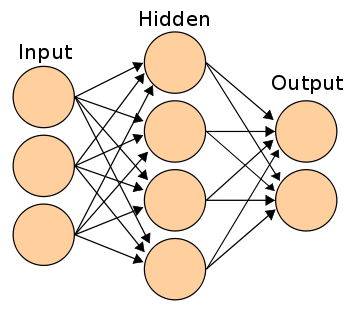
\includegraphics[width=0.8\textwidth]{ann}
    \caption{A simple representation of an artificial neural network}
    \label{fig:ann}
\end{figure}


Simple models often perform better when trained on bigger datasets
\cite{moreData} than complex models trained on much smaller sets. The N-gram
models, which is used notably in Natural Language Processing, is a simple model
that looks at N words at a time, and check if those words form a correct
sentence. It can be trained on very large datasets of sentences. It can
virtually be trained on all data available in this domain, which is about
trillions of words \cite{ngram}.

This is also true in image classification. Large and high-quality datasets of
millions of image are available to train the latest algorithm in image
recognition and classification. All this is possible thanks to the recent
explosion of data in many fields.

However, adding always more data may not result in better results. For certain
models, it can harm the predictive power of the network if the data is too noisy
or unlabeled. \cite{trainingData} Moreover, in certain domain like speech
recognition, the size of high-quality annotated speech retranscription is fairly
low, only just millions of word. Thus, more complex models are needed in order
to improve quality of the results.


\subsubsection{Progress in Models}

The progresses made in machine learning techniques and model are also
responsible for the last progresses we're witnessing. The back-propagation
algorithm, is a method to train neural networks in supervised learning, where
the desired outputs are known.\footnote{It can also be applied to some
unsupervised learning examples, which aims at finding unknown patterns in the
data.} It was first published in 1969 \cite{backpropagation}, and was applied to
the field of neural networks only in 1974 and later, before becoming one of the
most used technique to train neural networks.
%% redondant avec le texte
\footnote{\lq The most popular
method for learning in multilayer networks is called Back-propagation. It was
first invented in 1969 by Bryson and Ho, but was largely ignored until the
mid-1980s.\rq  \cite{RusselAI}}

We've seen that neural network can have one or more hidden layers. When each
hidden layer is used as the input layer for the next one, we can talk about
feedforward neural networks: There is no loop or cycle in the network. On the
contrary, recurrent neural network do present such loops. A neural network
will be qualified deep if it has more than two layers of non-linear neurons.
Deep learning has been highly popular recently, but it has been around since the late
80's. Yann LeCun successfully applied the back-propagation algorithm to deep neural
networks in 1989, in order to recognize handwritten zip Codes \cite{lecun}.
However the network was pretty long to train (about 3 days), and the lack of computing
power was one of the reason it took some time to become popular. It is now
used in domains such as image and speech recognition, as well as NLP.


\pagebreak

\subsection{Modern Models and their applications}

There are a various number of models in artificial intelligence and machine learning,
and they are evolving at a fast pace. Thus, we decided first to describe what a learning
agent is giving a general idea of what a IA software is, and then give a few
example of some recent models without entering in too much technicalities.

\subsubsection{Intelligent Agent}

The intelligent Agent paradigm is pretty recent in the history of Artificial
intelligence. It started to be accepted in the late 90's and was popularized by
Norvig and Russel \cite{RusselAI}. It is an attempt to encapsulate the various
problems encountered in Artificial Intelligence, from Graph exploration problems
like in chess, to the automated driving of a car. Thus, it defines Artificial
Intelligence as the study of intelligent agents.

 \lq An agent is something that perceives and acts in an environment. The agent
function for an agent specifies the action taken by the agent in response to
any percept sequence \cite{RusselAI} .\rq The environment as well as the agent
vary in form and complexity. Simple reflex agent, using defined if-then rules to
perform their actions will therefore be considered \lq intelligent\rq. Environments
can be extremely simple: a space of discrete positions for a player in a maze,
or very complex: a car evolving in the real world.

Intelligent agents can be classified in distinct categories:

\begin{itemize}
  \item Reflex Agents
  \item Model Based Agents
  \item Goal Based Agents
  \item Utility Based Agents
  \item Learning Agents
\end{itemize}

A model base agent will maintain a certain structure of its observable
environment, giving it more complexity than the reflex agent which does not
store anything about it. The goal based agent builds upon the model agent, but
tries to reach a certain goal (For example: Finding the exit of a maze, or
defeating the adversary in a Chess game), while the utility based agent is
optimizing a certain utility function along the path of its actions
\footnote{Utility functions come from the world of economics, and map states of
the world to a certain utility, giving a measure of the happiness of the agent}.
Finally, learning agents will explore their environment, and improve their
actions  by learning of their mistakes.

\subsubsection{Deep Learning}

We've already defined what deep neural networks was in the last section, neural
networks with 2 or more hidden layers. Deep learning refers to the use of such
networks in machine learning. Something important about Deep Learning is that
each layer get to have a certain representation of the data being learn. The
data is a composition of multiple factors, each factor being learned by a layer
in the  network. This can be particularly well observed in image recognition,
and was  recently demonstrated by Google in an attempt to better understand
neural networks:
\footnote{\href{http://googleresearch.blogspot.co.uk/2015/06/inceptionism-going-deeper-into-neural.html}
{Going Deeper into Neural Networks}}

\begin{quote}
  One of the challenges of neural networks is understanding what exactly goes on
  at each layer. We know that after training, each layer progressively extracts
  higher and higher-level features of the image, until the final layer
  essentially makes a decision on what the image shows. For example, the first
  layer maybe looks for edges or corners. Intermediate layers interpret the
  basic features to look for overall shapes or components, like a door or a
  leaf. The final few layers assemble those into complete interpretations—these
  neurons activate in response to very complex things such as entire buildings
  or trees.
\end{quote}

They managed to extract images from neural networks trained to classify images, by
giving them images of random noise and transforming them into what the network
consider to be a certain object. The figure \ref{fig:classvis} shows some example of
such image generation.

\begin{figure}[ht]
    \centering
    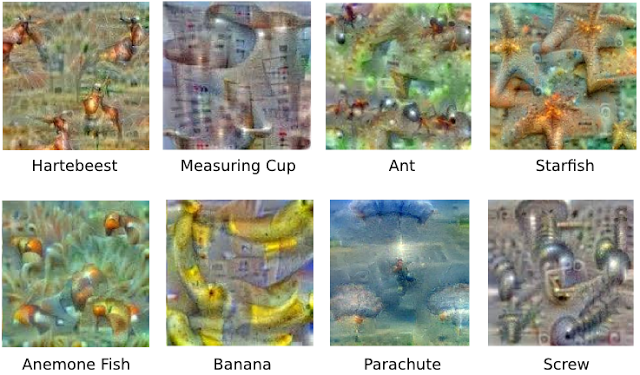
\includegraphics[width=0.8\textwidth]{classvis}
    \caption{Different classes of objects seen by a deep neural network}
    \label{fig:classvis}
\end{figure}

This gives insight on what the network actually learn, checking for learning errors
and gaining a better understanding on what's happening in the hidden layers.

They also fed images to the network, and extracted what was perceived in a
specific layer, amplifying what was detected. Low level layers amplify generic
features such as edges, contrasts or color-clusters. High-level layers have much
more precise representation of objects and complex features.

They also used this in order to generate image by recursively feeding the network with
an image, and selecting specific layers to amplify the results. The code for this
software, called deep dream, has been made public and a wide range of example are
available.
\footnote{\href{https://twitter.com/search?q=\%23deepdream&src=tyah\&lang=en}{Search DeepDream on twitter}}

\begin{figure}[ht]
    \centering
    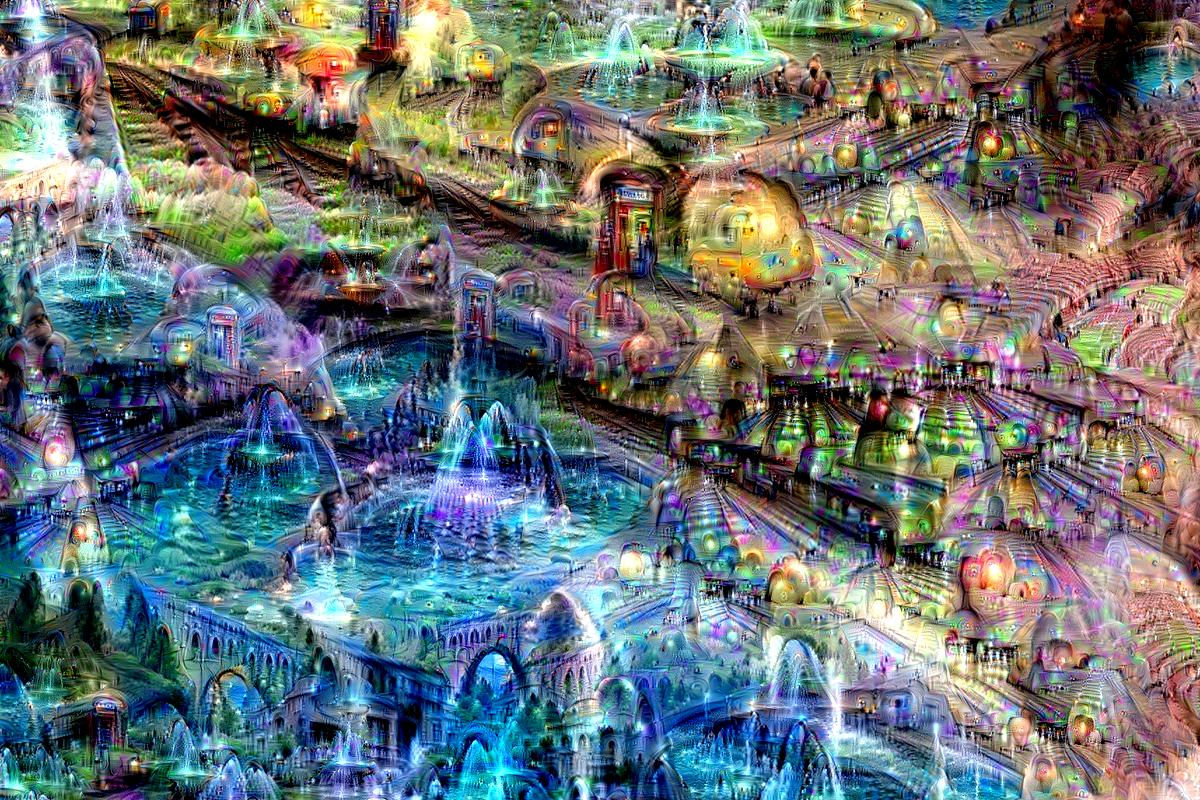
\includegraphics[width=0.8\textwidth]{deepdream}
    \caption{An image recursively generated from random noise on a neural network trained on architecture images}
    \label{fig:deepdream}
\end{figure}

\subsubsection{Word Vectors}

Word vector is a technique used to represent a set of words, or vocabulary, into
vectors. Some very interesting properties are captured into those vectors.

The first immediate result is that similar word tend to be clustered together:
Words which are semantically close end up to be close in the space of vectors.
\footnote{The popular \href{https://code.google.com/p/word2vec/}{word2Vec} tool provided by google gives some examples.}
Checking the closest neighbors of the word France will output a list of european
countries, the first being neighboring countries of France.

Another, less immediate result, is that it captures linguistics regularities
\cite{continuousWordVec}. The representation in term of vectors allows to make
some linear operations on the vector representations of words. For example,
the vector : $\vec{\textbf{King}} - \vec{\textbf{Man}} + \vec{\textbf{Woman}}$ will be very close to the vector
representation of the word \lq Queen\rq.

Figure \ref{fig:wordpair} shows some more example of such relationships. By
computing  the distance between countries and their capital, it can exhibit the
capital of other countries found in the training corpus. Some other examples
show grammatical similarities between words. The same distance is observed
between adjectives and their superlatives: small-smallest and tall-tallest.


\begin{figure}[ht]
    \centering
    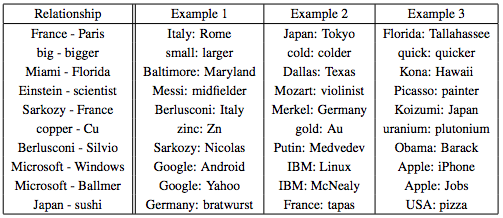
\includegraphics[width=0.8\textwidth]{vectors}
    \caption{Example of word pairs relationship. From {\em Efficient Estimation of Word Representations in
    Vector Space} \cite{wordVec}}
    \label{fig:wordpair}
\end{figure}

Word vectors need to be of high quality in order to be used in real world applications.
It has been used to improve machine translation \cite{translation}, and in sentiment analysis, which aims
at extracting subjective informations from the source.\cite{sentiment}


\pagebreak

%%%%%%%%%%%%%%%%%%%%%%%%%%%%%%%%%%%%%%%%%%%%%%%%%%%%%%%%%%%%%%%%%%%%%%%%%%%%%%%%
%%%%%%%%%%%%%%%%%%%%%%%%%%%%%%% Second Part %%%%%%%%%%%%%%%%%%%%%%%%%%%%%%%%%%%%
%%%%%%%%%%%%%%%%%%%%%%%%%%%%%%%%%%%%%%%%%%%%%%%%%%%%%%%%%%%%%%%%%%%%%%%%%%%%%%%%


\section{The impact of AI on the entrepreneurial ecosystem}

Now that we've seen the improvements of AI technology, we're going to look at
the impact those technologies can have on the entrepreneurial ecosystem.
Our approach will be the following: we'll explore a few applications of AI
technologies, and propose startup ideas related to this.

Of course, some companies, including startups, are already leveraging the latest
progress in AI to offer a commercial service, or are expected to do so.
We'll therefore start by reviewing the first AI commercial progress in the
space. Then, we'll look at other area to expend our analysis

\subsection{Impact on startup ideas}

\subsubsection{Self-driving cars}

\paragraph{A bit of context}

The first autonomous cars appeared back in the 1980's with the Canergie Mellon
University Navlab project in 1984, and a similar project by Mercedes Benz in
1987. Those project were were considered pure exploration at the time.
But things have changed. In 2005, DARPA launch a Grand Challenge which was won
by a team of engineers at Stanford, who created a first self-driving car
prototype. Since then, the team has been hired by Google to create the first
autonomous that has started hitting the road of California in the spring 2015 \footnote{\href{http://www.google.com/selfdrivingcar/}
{Google car}}.
A few others are following this way: Uber \footnote{\href{http://www.businessinsider.com/why-uber-is-investing-in-autonomous-cars-2015-8?IR=T}
{Why Uber is investing in autonomous cars}}, Tesla and potentially Apple to name
a few.

\paragraph{Technology behind those cars}

Let's look at the technology behind those.

First, autonomous car include a ton of sensors to gather data about their
environment. Let's look into those.

The position of the car is determined with a classic GPS, to which are added
tachometers, altimeters and gyroscopes to enrich the only GPS data. Then come
radar sensors that are located all around the car to localize potential
obstacles. Usually, there are 4 of those: 3 at the front and 1 at the back of
the car. On the sides of the car, there are ultra sonic sensors which are a bit
different, they're used to locate objects close to the car. Think about parking
for instance. When you think about it, all this information gathered by these sensors,
if properly interpreted, will give far more precision and safety to an autonomous car
than a regular car driven by a Human.

\noindent On top of this, a video camera points to the front. It aims to detect
traffic lights and road signs. The central element among all those sensors is
the LIDAR: Light detection and ranging. This element is located at the top of
the car. It identifies the edges of the road, and provides a 360 projection of
the environment around the car.

\smallskip

\begin{figure}[ht]
    \centering
    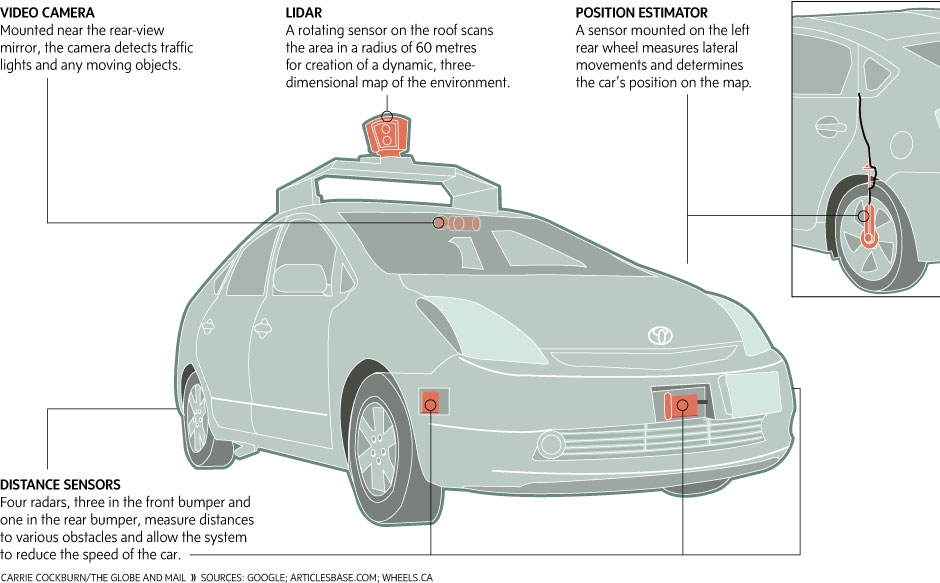
\includegraphics[width=\linewidth]{car-diagram}
    \caption{A self-driving car and its sensors}
    \label{fig:car}
\end{figure}

\smallskip

Second, the car includes a powerful computer to analyze all these parameters
and actually \lq drive\rq the car. Let's take the example of Google's software
called \lq Chauffeur \rq . It's composed of two parts. One is hard-coded
(road signs, traffic lights colors), and one is a learning part. Every mile is
logged and provides additional data on how the car should drive itself.
Therefor, the car is able to predict the behavior of surrounding elements
(both car, bikes, pedestrians). Such things are based on \gls{neuralLabel} being
fed with the driving data of million of other cars
that Google has been collecting. This video by Google provides a great example
of how the car perceives its environment and can make decisions.

\smallskip

\begin{figure}[ht]
    \centering
    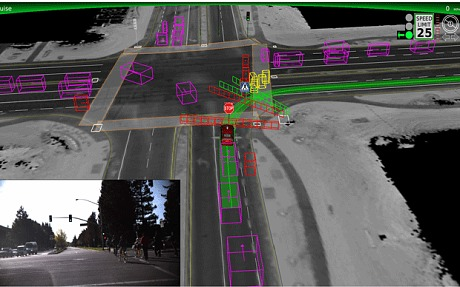
\includegraphics[width=\linewidth]{google-car}
    \caption{How the Google car perceives its environment.
    \href{https://www.youtube.com/watch?v=dk3oc1Hr62g}{More in this video}}
    \label{fig:google_car}
\end{figure}


\smallskip

\paragraph{Car industry disruption}

The disruption is happening at several levels: some startups are building add-ons
to current cars, so they can get self-driving functionalities. For instance,
a Californian company called Cruise
\footnote{\href{http://www.getcruise.com}{Cruise Website}}
enhances a car's capabilities by seamlessly integrating self-driving car
capabilities to your existing car. It works by adding sensors and a computer to
the car, and works in a similar fashion as the Google car. The idea is that you
can add those features to your car for about \$ 15,000 depending on the vehicle
you have. Google has a similar approach: according to several journalistic
sources, they intend to resell their self-driving technologies to automotive
companies. Though, many people fear that Google will have a significant
bargaining advantage, as those car companies don't have the technology yet.

Some other companies intend to replace current car makers. Tesla is the best
example in the category. Though the company CEO, Elon Musk, is confident
self-driving cars will hit the market by 2020, there were no public statement
about Tesla building such cars. \footnote{\href{http://my.teslamotors.com/fr_CH/forum/forums/tesla\%E2\%80\%99s-musk-sees-fully-autonomous-car-ready-5-years}
{Elon Musk sees fully automated cars in 5 years}} In a recent video, he was asked whether Tesla
would be willing to provide Uber with self-driving cars, and declined to answer.
Many reporters concluded that Tesla will likely be the first company to sell
autonomous cars, that were built in-house. Similar to Tesla, there could be new
car giants rising by leveraging the opportunity to build both a new type of car
and a powerful self-driving technology. \footnote{\href{http://www.forbes.com/sites/chunkamui/2014/08/04/5-reasons-why-automakers-should-fear-googles-driverless-car/}
{Five reasons why automakers should fear Google's driver less car}}

Finally, the most ambitious model is probably the one by Uber. The idea behind
it is that using UberX costs about \$ 2.15 per mile (source: AKA research).
Owning a personal car is \$ 0.76. Uber wants to create Car-As-a-Service.
The idea is similar to what Uber is today, but without the drivers. Think about
it for a moment. The car driver accounts for most of the cost of an UberX ride.
Therefore, if you can remove the driver, the cost would be \$ 0.25 per mile.
It's not only about replacing the driver, it's about making the car available
for customers at any time, on any day. Whereas a driver takes some rest and
parks their car, a self-driving car could be on the road almost 24/7.

\medskip

\begin{figure}[ht]
    \centering
    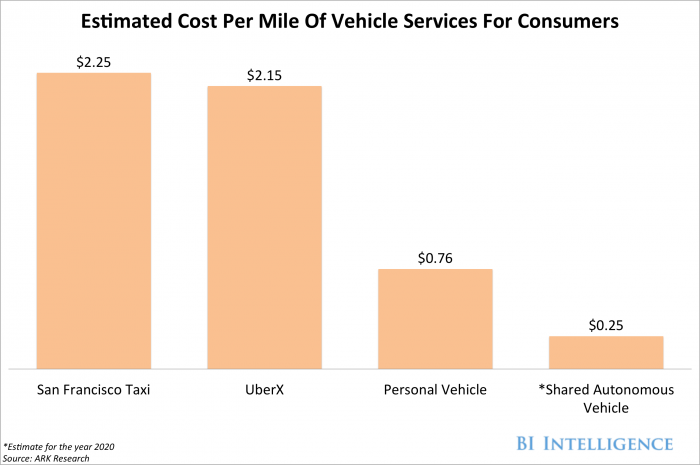
\includegraphics[width=\linewidth]{vehicle-cost}
    \caption{Cost of a car per mile for different scenario}
    \label{fig:cost_of_car}
\end{figure}

\smallskip

No matter who's leading that change, it's likely that our own definition of the
car is going to change. Mercedes has shown an example of a car being similar to
a living room: the Mercedes-Benz F 015. Travelers could sleep, chat, browse the
Internet as if they were at home. The car has been driving around San Francisco
this year.

\smallskip
\begin{figure}[ht]
    \centering
    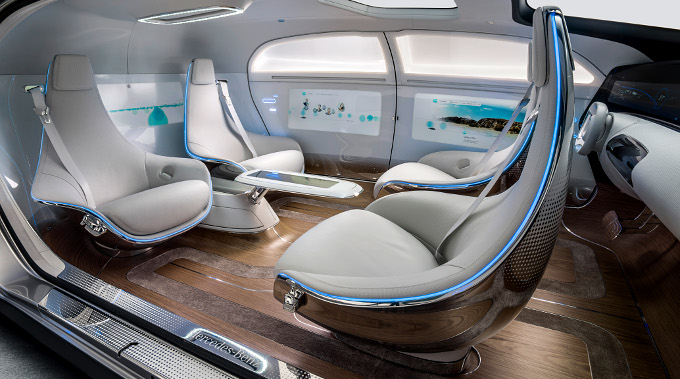
\includegraphics[width=\linewidth]{mercedes}
    \caption{\href{http://www.entrepreneur.com/article/243751}
    {Mercedes Benz F 015 A driving living room}}
    \label{fig:mercedesBenz}
\end{figure}

\smallskip

Another big change would be the oil station network. Since the car could drive
themselves to refill, or could be fully electricity powered, it will most likely
be the end of oil stations as we know them. Those will be probably automated as
well, and moved to non-residential areas.


\subsubsection{Speech \& natural-language recognition}

The speech recognition movement has been initiated to the large public with a
startup bought by Apple, Siri. This startup was initiated a DARPA project as
well named CALO. Essentially, it works by transcribing speech to text, and then
parses the text to perform actions. Google has launched a similar service called
Google now. Both these system can perform actions based on the user's speech.
This technology enables the user to perform actions on the service of his
choosing (OpenTable, Yelp), without having to use any interface. The speech is
the communication tool.

\\

\paragraph{Technology behind it}
Personal assistant technologies rely on three parts.
The first one is about extracting the meaning of the speech to figure out which
action to perform. In that case, Siri uses for instance part of speech tagging,
noun-phrase chunking, dependency \& constituent parsing. On the other side,
such service should plug into third party services. The complexity lies in the
ability to connect with very various systems (AirBnb, HotelTonight, Couch-surfing
,Bookking.com only to make a hotel reservation). Once this has been done, Siri
needs to communicate back with the user, converting API responses to oral \&
human communication.

\paragraph{Use cases}

Plenty of services have followed the Siri path, usually in a more advanced
fashion. It's interesting to note that some services are built with technology
at its core (Siri \& Google Now), whereas others are human-based at first. The Y
Combinator startup called \lq Magic\rq  is the exact opposite. The service only
includes the written language recognition. For instance, a user can text Magic
asking for anything they'd like, and then the service will connect to third
party services (in a similar fashion than Siri) to provide the service live. The
complexity therefore lies on relying on a very large number of 3rd party
services to provide a very large offering to the user. When a regular supermarket
has a limited inventory, Magic, as a personal assistant, needs to be able to
deliver anything the user wants. The second part of the complexity is scaling.
When you have human handling each operation at the beginning, you need to
progressively create processes to better handle certain tasks, and eventually
automate entire parts of the workflow.

Combining AI and diversity of requests doesn't seem to be possible today. Such
startups are having trouble to scale. The current solution is to combine a mix
of the two. Facebook Messenger recently launched a service called M that
illustrates it: they've leveraged the purchase of the French startup Wit.ai and
a team of personal assistants that handle manually some request to provide this
personal assistant service.

This market is likely a winner takes all one. Since these personal assistant
platforms are about connecting people with services, their model is similar to
Google's search engine. If you are the entry point for the customer, it's very
hard for competitors to make the users switch. Startups like Magic benefited
from their speed of execution, but the ability to scale requires to leverage AI
technology. It's not clear today whether startups or giants will succeed in that
field. Though it's interesting to see that the 2 opposite approach are now converging
to a similar solution.

Additional services from startup in that space intend to focus on one vertical
only. A good example of it are personal assistant focused on organizing meetings
between to person who want to schedule an appointment. To name a few, players in
that space are x.ai, assistant.ai or Juliedesk. These companies are managing to
live up to their promise, but the complexity once again lies in the ability to
scale. They are strongly investing in AI to replace human services that they
first relied on.

Finally, we could imagine two models for that space.
One would be a model built by a major tech company (among Facebook, Google or
Apple) that would provide any kind of service by levering a strong AI
technology, and would plug into a very large number of APIs from company that
provide food delivery, order delivery, or pretty much anything.
The second model would be a platform one. A company like Magic could be the
entry point for the user. Then, if a calendar request is made to Magic, it would
just have to tag it as so and to route it to a Calendar booking service such as
x.ai.

The former seems more likely as concentrating the efforts in Machine Learning is
probably the best approach to achieve the best results, though the two are
possible.

\subsubsection{Death of interfaces}

The most natural interface of communication between Human beings is the spoken language.
Other forms of interface were created to allow people to use machines in the simplest way as
possible. However, an interface, even if well designed, will never be as immediate and
easy to use as spoken language.

Consequently, the main benefit of a personnal assistant for the user is that it's a very easy way to
communicate with a machine, in order to get a service. Think about the
User-Experience behind it. If you use a speech recognition, you would just
have to say: \lq Book me a table for 2 in a historic area of Paris, where I
can eat Italian
food.\rq. That will do the trick.
If the user was to do it on their laptop or on their phone, they'll need to:
\begin{itemize}
  \item Find the right service to search on (TripAdivisor, OpenTable, Yelp?).
  \item Perform the search.
  \item Make a choice
  \item Go through the reservation process.
\end{itemize}

The former is way faster. Another benefit is in what we would call \lq unique\rq
cases. Say you want to book a laser-tag party in Paris, and you've never done it
before. You don't know where to look, so you're going to spend time figuring out
how to book a good laser-tag game. You'll probably need to benchmark a few,
look at the review, etc.

A strong case in favor of speech-based application is that you don't need to
learn about the existence of the service, and you don't need to use any
interface. UX designers often struggle to make an app available to all. No
interface is probably the most efficient. Even a 80 year-old who has never used
an app in their life would be able to use it. We can then imagine that, instead
of having dozens of apps on our phone or dozens of websites pinned on our
browsers a single personal assistant app could do the job. Just like Google
does for search today. This user experience part make those personal assistant
particularly appealing in the long-run, because the friction to start using them
is very low. A good example of it we saw is about forwarding professional
expenses to the company's accountant. The mainstream service for it today is
Expensify. You just need to install an app on your phone (meaning, if you have
1000 people in the company, they all need to install it), then you can take a
picture of a receipt and it will automatically be sent to the company's
accountant. Right now the picture is manually treated behind the scenes, and the
process is only half-automated, taking several hours to process a picture.
This would be a lot easier with a speech or written language
recognition app. You could just send over the receipt's picture via text to the
company AI bot. It will recognize what it is, potentially ask a few question
about the expense and done.

Time will tell, but usually the service that provides the simplest user
experience wins. And it's likely that the personal assistant user experience is
the simplest.


\subsubsection{The next generation of SaaS}

A new generation of SaaS is on the rise. The current SaaS solutions are
comparable to toolboxes. They offer the ability to perform any action on any
object. For instance, in the Salesforce interface (a CRM in SaaS for Sales
people), you can basically customize the interface as much as you want so you
can display any piece of information about a prospect.


\smallskip

\begin{figure}[ht]
    \centering
    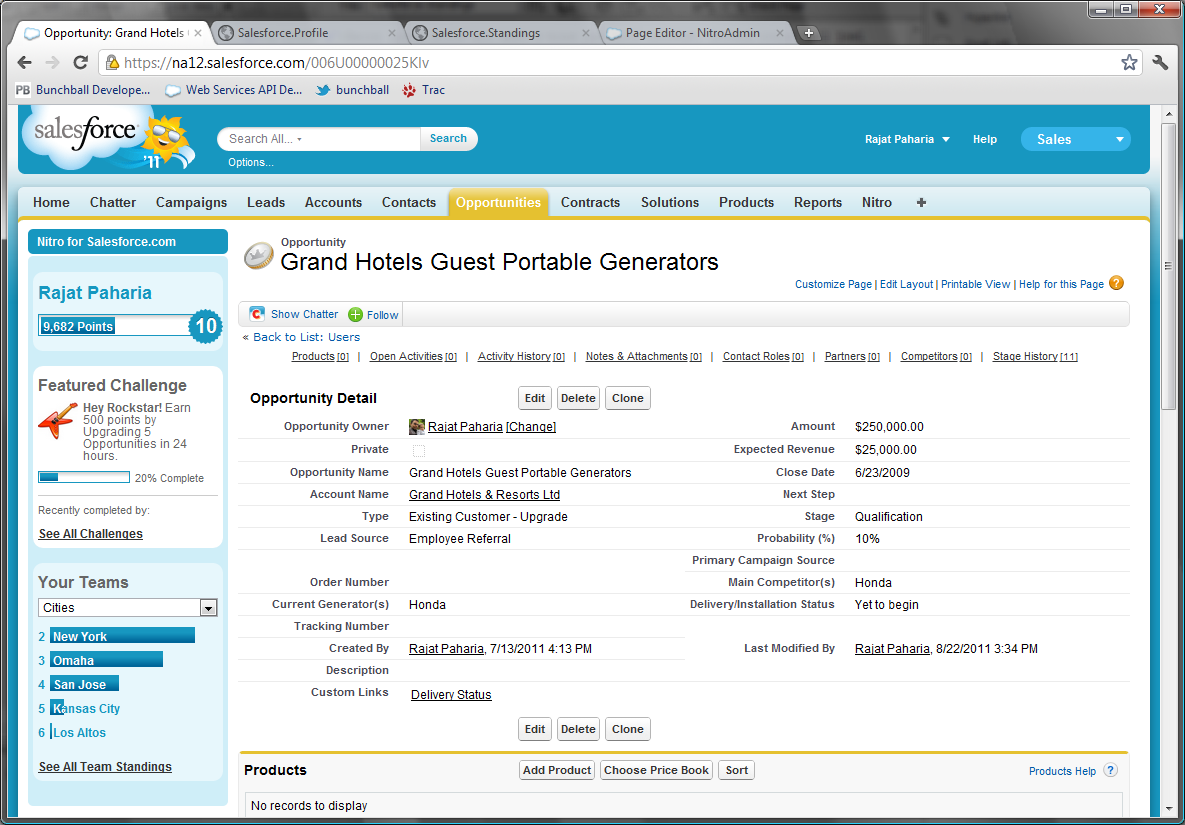
\includegraphics[width=\textwidth]{salesforce}
    \caption{Salesforce's prospect interface}
    \label{fig:salesforce}
\end{figure}

\smallskip

The main challenge with those interfaces is that they end up being very crowded.
There a second issue. The more information there is, the more complex it becomes
to identify that you should perform an action. Say one of the metrics you use to
track the customers usage of your application goes down. You may have a hundred
metrics and miss this. Therefore, you won't be able to notice it. SaaS CRM are
great to manage a very large number of customers, but that comes with a price.
The ability to pay a lot of attention to a given customer doesn't scale that
easily.

There are some solutions. CRM like Salesforce, Zoho CRM, Zendesk and others
provide the ability to create rules to identify specific behavior, so the user
can be notified about certain events. Say a customer is about to churn because
metric X is low, the sales rep will get a notification and will email the
prospect. All this sounds like it could be a good candidate for machine learning
right? It is. A new generation of SaaS software is on the rise. This generation
uses machine learning to automate those patterns. Essentially it can do two
things: 1. is improving the user experience, and 2. is helping the user in
regards to what to do to reach their goal.

\paragraph{Smart interfaces}

First, the user experience. We've seen that the interface of the current SaaS is
usually crowded. That negatively impacts the productivity of the user, because
they need to find the right piece of information they need among a ton of pieces
of information. How could that be easier. Let's take the example of Zendesk,
which is a CRM for customer support. Essentially, Zendesk is designed to respond
to customers' inquiry, and to make it easy to satisfy those customers. The thing
is, there are a ton of information, both available inside Zendesk, or in 3rd
party services (e.g. the payment platform the company uses). Therefore, the
customer support person needs to look around for the right piece of information,
which takes time. Machine learning can help here. Companies like Gorgias.io, or
Wise.io already display specific contextual buttons for the user to take actions
according to the content of the message.

\smallskip

\begin{figure}[ht]
    \centering
    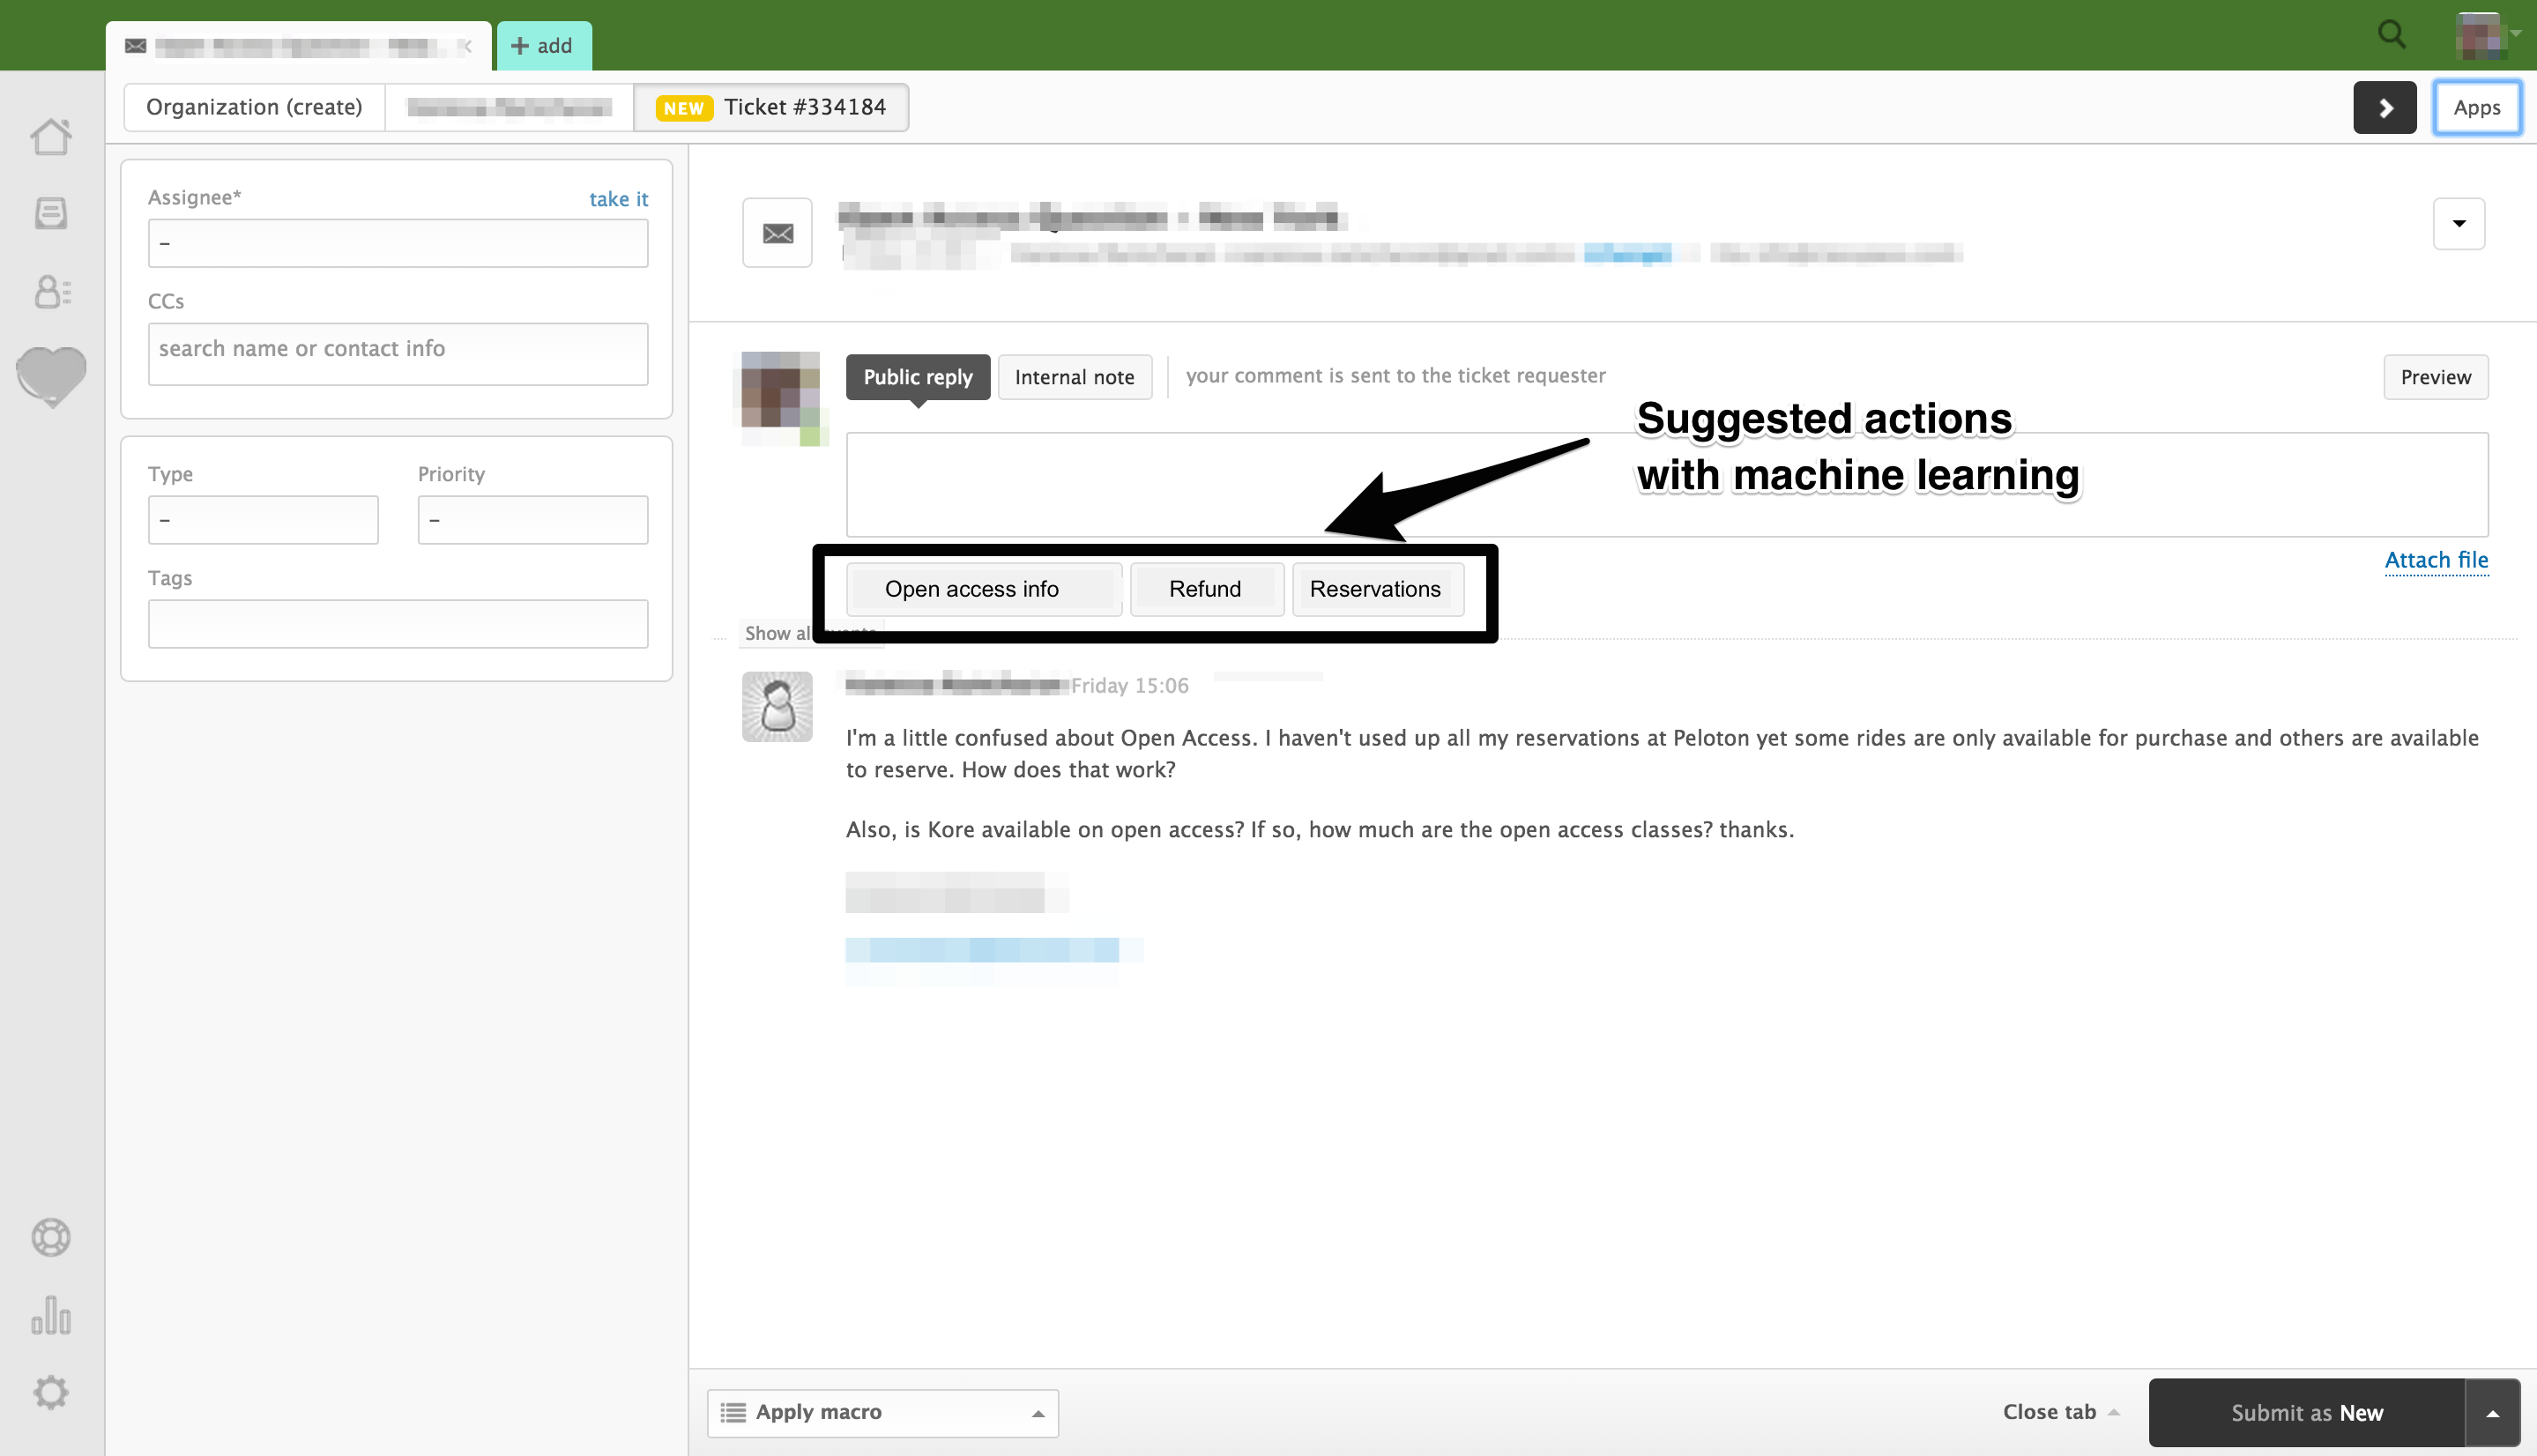
\includegraphics[width=\textwidth]{zendesk}
    \caption{Gorgias can suggest the right canned response to a message}
    \label{fig:gorgias}
\end{figure}


\smallskip

It means when responding to a message, the support person doesn't have to look
around for the right canned response. They are just suggested it by those smart
pieces of software. It could be the same with the information displayed in the
interface. A customer request contains a large amount of information, that can
help identify what piece of information will be needed by the customer support
person to satisfy the request. On top of this, customer support is usually
receiving hundreds of requests per day. Therefore, their could be tools that
only show the right piece of information to the user, based on what is needed to
resolve the case. One step further would be to suggest the right piece of
information to the customer.

\paragraph{Suggestions of actions}

Second, we can expect the next generation of software for Enterprise businesses
to be able to suggest actions and identify patterns by itself.
\footnote{\href{http://techcrunch.com/2015/07/27/the-next-wave-of-enterprise-software-powered-by-machine-learning}
{TechCrunch Enterprise Software powered by machine learning}}
These services will be based on the collection of very large amount of data about
a given customer. Then, it will be able to identify actions to be made in regards
to the customer. A good example of it is identifying that a customer is ready to
buy. A few SaaS services already provide that kind of intelligence:
\href{http://www.gainsight.com/}{Gainsight} and
\href{http://uk.insidesales.com/}{Insidesales} are good examples of it.
The main challenge they have is that they work as plugins. Therefore, their
service is great, but cannot impact the user experience of the sales person
inside Salesforce for instance.
We can expect the next move in that sphere to be for Salesforce to integrate
those capabilities. There are actually two ways to integrate them. The first
is to add even more information in the interface to suggest or show those smart
pieces of information / those suggestion of actions. The second is to integrate
them in the user flow. Let say a user needs to send an invoice to a customer on
a monthly. Salesforce could identify this, and figure out that customers who
receive also stats usage while getting the invoice are less likely to churn. In
that case, the software could suggest to not only send the invoice, but also
send monthly usage statistics along with it, in the click of a button.
It's likely that unifying the user flow, which means the current course of
actions the user takes in Salesforce, and the suggestions from machine learning
algorithm would be the best way for users to adopt and use it. Therefor, the
value will be captured by the companies which manage to unify machine learning
suggestion in the current user flow.

\subsection{Impact on startup structures}

\subsubsection{The path to the full-software company}

If you look at how a SaaS business works today, you'll realize that the company
essentially relies on a very large number of other SaaS services. For instance,
it will use a SaaS platform for analytics (MixPanel, Kissmetrics, another for
marketing (Marketo, Customer.io), another for CRM (Intercom, Salesforce) another
to handle payments \& accounting (Stripe, Octobat, Baremetrics), etc.
All this demonstrate one reality, each business unit in the company has its own
SaaS platform, and they are all inter-connected. The step one was to provide
each of those business units with a tool that facilitates their life. Step 2 is
to automate those business units. A good example of it is Stripe, Baremetrics
\& Octobat. Those three SaaS combined can almost take care of all the payments,
invoicing and sales reporting, without requiring a heavy setup nor human
intervention once they work. Octobat automatically invoices the customers
according to the payments which were made or which are scheduled in Stripe.
Baremetrics does the reporting out of the box.

\begin{figure}[ht]
    \centering
    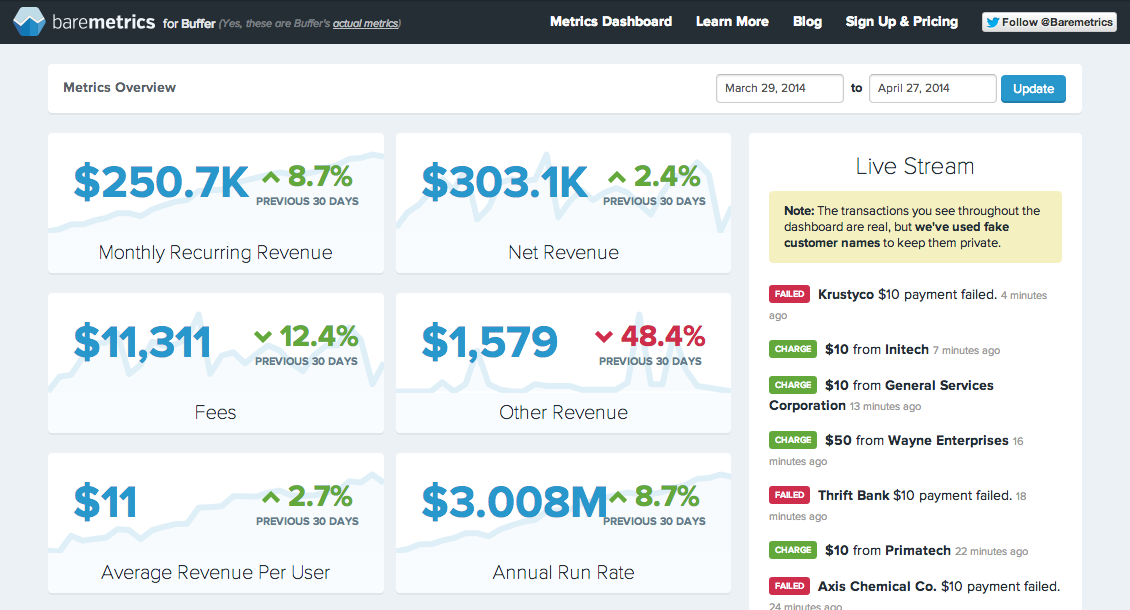
\includegraphics[width=\textwidth]{baremetrics}
    \caption{Baremetrics provides business analytics out of the box for the
    company manager to monitor progress.}
    \label{fig:baremetrics}
\end{figure}

\smallskip

One can guess that this behavior will expend to other areas of the business,
that will be fully automated. Some people think it will only apply to blue
collar work. But that's not the case. Project management can also be automated.
Tools like \href{https://www.mturk.com/mturk/welcome}{Mechanical Turk} by Amazon
enable to distribute work to remote contractors, and to achieve big projects at
scale. Researchers have worked on a experiment: a basic AI software had to
conduct a project from Scratch with this platform, by splitting the general
task into small pieces that it hired contractors to do. This is probably also a
glance at the future of a company: middle management will be automated.


\paragraph{The Uber example}

Probably the best example of this is Uber. A blog post by Peter
Reinhardt\footnote{\href{http://rein.pk/replacing-middle-management-with-apis/}
{Replacing Middle Management with APIs}} demonstrates that a big trend among
tech businesses is to automate workloads distributions. Uber does it by
providing end users to directly order a cab. If you think about the experience
from the taxi driver experience, their workload is totally automated. They are
assigned rides by Uber's algorithm, which they just need to execute. Same goes
with other kinds of contractor work, for instance
\href{https://www.getbannerman.com/}{Bannerman} provides the ability to book
security guards on demand, without the middle man.


\begin{figure}[ht]
    \centering
    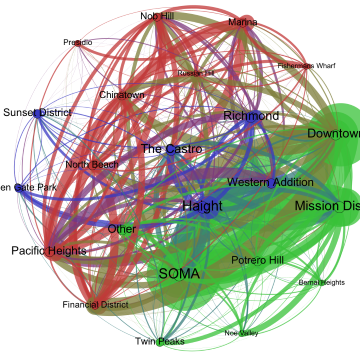
\includegraphics[scale=0.8]{uber-graph}
    \caption{Uber's traffic predictions}
    \label{fig:uber-graph}
\end{figure}

\smallskip

Uber can predict taxi traffic based on historical data, and suggest drivers to
go to the right place. This
\href{http://blogs.mathworks.com/loren/2014/09/06/analyzing-uber-ride-sharing-gps-data/}
{graph} shows the rides made by Uber drivers on weekends in San Francisco.

The size of the nodes represent the number of rides per location, hence their
popularity. The colors (green, blue, red) show which cluster a node belong to.
Hence, you can predict in which area a taxi driver will drive: we'll most likely
stay in the same cluster, and distribute the work accordingly.

\smallskip

\paragraph{How to achieve a full-software company}

There are two challenges related to building a full software company. One is the
ability to build a software for each business unit. We've seen that the startup
ecosystem is making progress in that direction: Uber is doing it for the taxi
workload management, Octobat for invoicing software. We can expect to see more
and more pieces of software handling part of the business. The second aspect of
it is the ability to gather and share data. For a piece of software to do the
full job of a business unit (say: accounting), the software needs to have access
to all the data related to the business. Usually, this data is manually shared
between services. To automate the process of sharing information, there's a need
for a software that fully handles it.

We're good progress here. A company like
\href{https://segment.com/}{Segment.com} handles it for analytics and user
activity data. The admin just needs to install Segment on their website and
define user events. Then, it will share this user data among a large amount of
third party services through API integrations built by them. The user just need
to activate a service on Segment for the data to be shared. It's that easy.

\smallskip

\begin{figure}[ht]
    \centering
    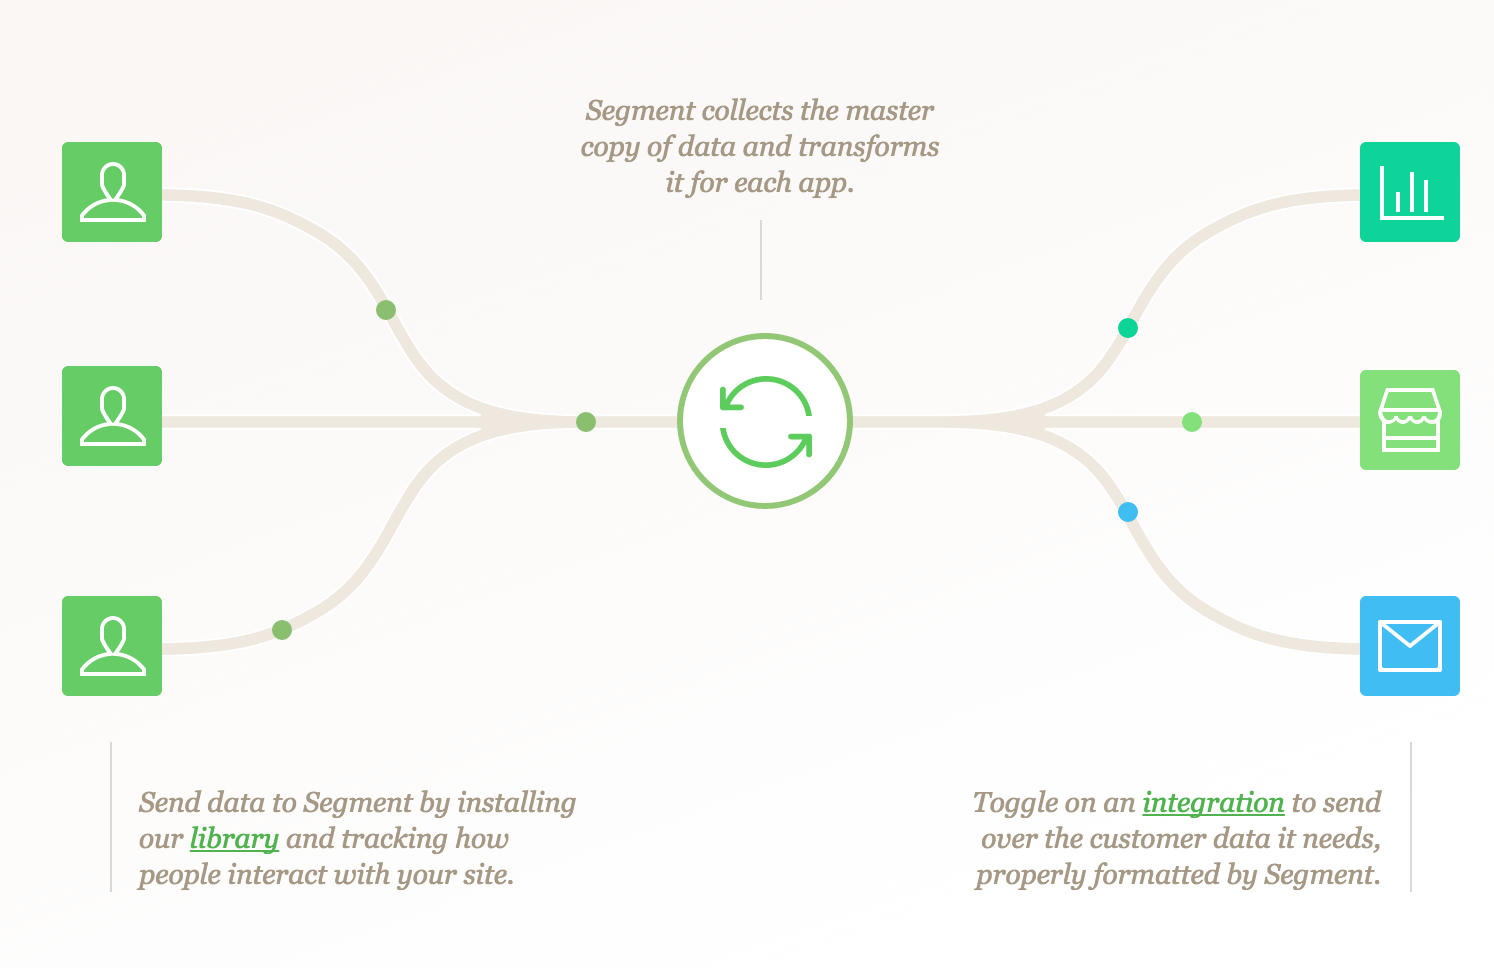
\includegraphics[scale=0.5]{segment}
    \caption{Services like Segment share data among all software a company has.}
    \label{fig:segment}
\end{figure}

\smallskip

We can expect to see similar services at the scope of the whole company. Think
about the ability for a software not only to have access to any piece of
information about users or about the business, but also to be able to perform
actions in third parties. Today, we're at the information sharing step, but soon
we'll reach the latter. Once it's possible to both share information and perform
actions (e.g. offer them a refund after they experience a bug or raise a
complaint), we'll reach one step further in the fully automated software
company. The human work may then focus on the creativity aspect of it, while it
will be possible to fully automate the operational side of things.

\subsubsection{A shift in pricing and business models}
The current business models in the startup ecosystem are the following:
\begin{itemize}
  \item Charge to the end user
  \begin{enumerate}
    \item Monthly subscription (SaaS B2B, Media, etc.)
    \item Upfront cost (software)
    \item Transaction fee / usage fee
  \end{enumerate}
  \item Charge to a third party (mostly advertising)
  \begin{enumerate}
    \item Monthly subscription (SaaS B2B, Media, etc.)
    \item Transaction fee / usage fee
  \end{enumerate}
\end{itemize}

 In the last 10 years, we've seen a strong shift from upfront cost to monthly
subscription \& usage fee. A good example of is the Adobe suite. It was priced
per version until 2013 when they started charging per month, shifting to a SaaS
business model. The latter (subscription and usage fee) are aligned to the
payer's interest: you pay as you use the service, which means you pay as you
get value from it. These two models tend to be ideal because of the mere fact
that they are aligned with the user's interest. One can note that usage fee is
the best aligned of the two, and therefor the one companies favor. The
challenge is that to price your service according to usage, you need to show
that usage directly impacts the customer's interest. Let's take the example of
a recruiting platform. Some companies like Job boards enable you to post a
listing for a job offering online. You pay a subscription: 1 listing for a
month costs a certain price. Whereas the customer's interest is to hire the
right person for that job, not to post the listing. As software gets better,
and as automation and communication between pieces of software increases, it
will become easier to evaluate the performance of this job listing by the
quality of applicants to that jobs. Therefore, the model will change from
subscription to usage fee, where the usage is aligned with the benefit you
expect from the service. All this suggests that services like recruiting will
be split into smaller services (job broadcasting, candidate screening with
machine learning) that will enable to price based on what's considered has
performance, in that example successfully hire someone. We can expect the
general trend of having software automatically performing tasks and of
providing objective stats on its performance to lead to more customer-driven
business and pricing models.

\pagebreak
%%%%%%%%%%%%%%%%%%%%%%%%%%%%%%%%%%%%%%%%%%%%%%%%%%%%%%%%%%%%%%%%%%%%%%%%%%%%%%%%
%%%%%%%%%%%%%%%%%%%%%%%%%%%%%%% 3rd Part %%%%%%%%%%%%%%%%%%%%%%%%%%%%%%%%%%%%%%%
%%%%%%%%%%%%%%%%%%%%%%%%%%%%%%%%%%%%%%%%%%%%%%%%%%%%%%%%%%%%%%%%%%%%%%%%%%%%%%%%


\section{The limits of Artificial Intelligence}

\subsection{Technical limitations}

\subsubsection{Limits in models}

Though some impressive results have recently been achieved with deep neural
networks, there are still hard to train, and fine tuning the weights and
parameters between the unit of the network is more of an art than a science.
When applied to image recognition, it is possible to visualize what are the
different features learned by the layers of the network, but is is hardly the
case with speech recognition and natural language processing.

Moreover, some limitations has been discovered in deep neural networks
\cite{deepLimits}. It is possible to slightly alter a image that is correctly
classified by a network, so that the two images are indistinguishable to the
human eye, but differ in classification for the network.

\begin{figure}[ht]
    \centering
    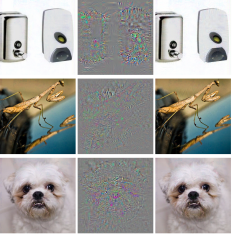
\includegraphics[[width=0.7\textwidth]{adversarial2}
    \caption{Left is the correctly classified image. In the center is the difference
    between the two images, magnified by 10X. Right is the miss-classified image. }
    \label{fig:adverserial}
\end{figure}


\subsubsection{Computing limitations}

We've seen that hardware progress was responsible for some of the major
progresses  made recently. However, we're still far behind the capacity of human
brain in terms of computing power, as the fastest computer in the world is
equivalent to $1\%$ of  our brain. There are some concerns on the power required
to run those machines. This super computer uses about $20MW$
(principally due to the cooling system), while our brain runs on only $20 W$.
Some
attempts have been made at creating efficient low-energy computer, notably by
Pr. Kwabena Boahen at Stanford. He created a computer mimicking the brain made
of 16 Neurocore, each costing about \$40000,  resulting in a something \lq 9,000
times faster and using significantly less power than a typical PC\rq.
\footnote{\href{http://news.stanford.edu/news/2014/april/neurogrid-boahen-engineering-042814.html}{Stanford
bioengineers create circuit board modeled on the human brain }}

\subsection{AI represents a major challenge for startups and for the society}

\subsubsection{AI and Machine Learning are reshaping the job market}

\paragraph{Some jobs will disappear}

As machine learning makes progress, it can automate things that were made by
human in the past. Again, a good example of it is the car industry. While it's
probably a good thing for anyone to not have to drive your car to work, it gets
much worse if you're a taxi driver and work to pay the university fees of your
children. Car drivers are we know them are likely to disappear one day, and this
day is not that far. The French car company Valeo states that there are 4 steps
from manual driving to fully self-driving cars. One is support to park your car.
Two is a car that can park itself after you've brought it next to a parking
slot. Three is a car that you drop next to a parking, and that can find its way
to the parking spot itself. Four is the fully self-driving car. We're already at
step two. The company predicts that we'll be at step 3 in 2020, and step four in
around 2025. What's the impact? People who drive car for a living will lose
their jobs. Along with truck drivers. Along with people who work in oil
stations. Along with small towns which only exist because of car or trucks
stopping by to rest. It's likely that some restaurants or motel nearby the road
will disappear. That's just the example of the car industry. A ton of other
industry will be impacted: industrial workers, office and administrative
support, transportation, construction, etc.

\smallskip

\begin{figure}[ht]
    \centering
    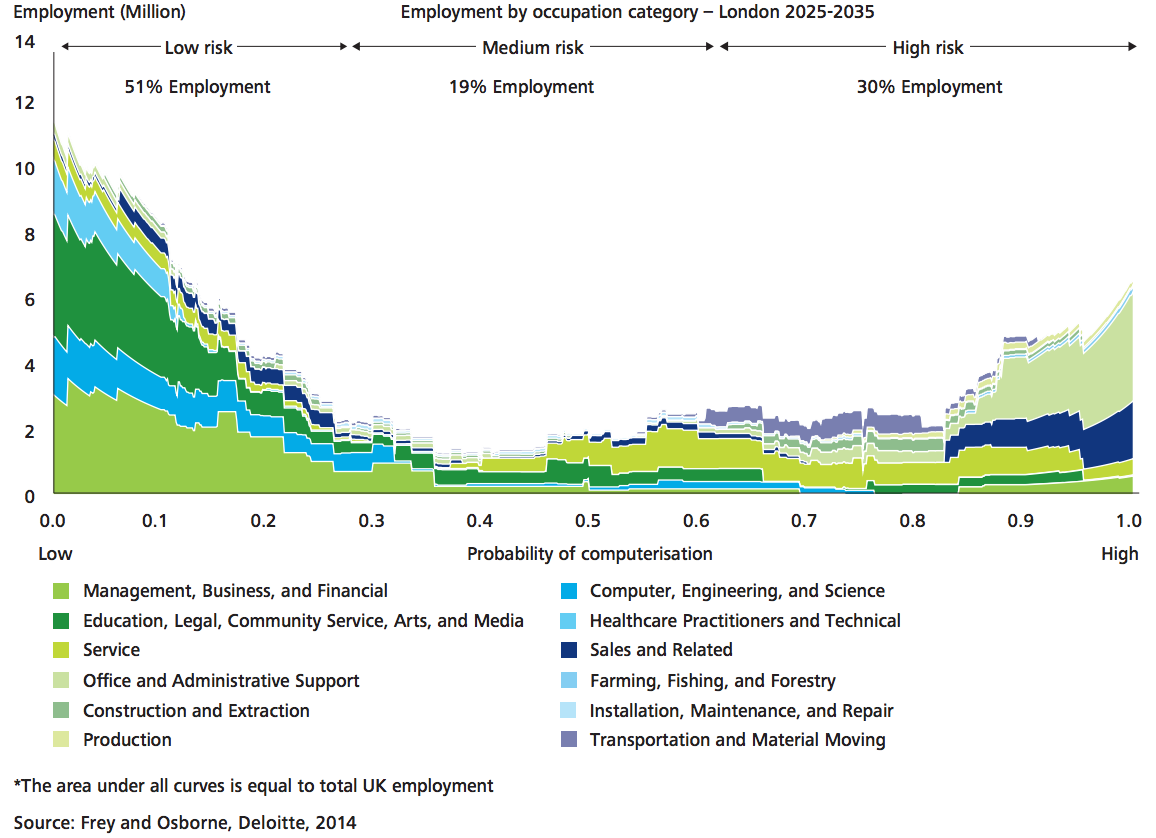
\includegraphics[scale=0.6]{jobs}
    \caption{\href{http://www2.deloitte.com/content/dam/Deloitte/uk/Documents/uk-futures/london-futures-agiletown.pdf}
    {Study by Deloitte on jobs in at risk from automation}}
    \label{fig:deloitte}
\end{figure}

\smallskip

Usually, those who protest against that trend have to face the fact that
technology is creating more jobs than the number of jobs it destroys. Though, a
\href{http://www.pewinternet.org/2014/08/06/future-of-jobs/}{Pew Research article}
states that for the first time, experts consider that by 2025, technology will
destroy more jobs than the number of jobs it creates. It's a widespread trend to
think that this will mostly impact blue-collar jobs. Though, it's likely that it
will impact white-collar as well. We've looked into it: management-related tasks
can for instance be automated. Lawyers, accountants, financial people, traders will
most likely suffer the impact of machine learning progress as well.



\paragraph{A change in the way we work}

We can expect the way we work to change as well, though in positive fashion.
White-collars today spend a lot of their time working in front of a computer.
Progress we've analyzed before in the NLP area will reshape the way we work. For
instance, most communication is currently handled through written form, we
basically communicate with our keyboard for work. NLP can enable a change here,
we'll be able to work using our voice to virtually communicate (as we currently
do with emails). This is an example of the positive impact machine learning can
have on jobs, increasing worker's productivity.

Those changes lead to two major challenges for our society. One is about
reshaping the way we work. Two is about enabling people to work.

\subsubsection{New social rules}

Since we can expect technology to start destroying jobs by 2025, we'll need to
rethink the way society works. Today, work is the core element of the society.
Unemployed people are helped to find a job. We study to find a job. Social
classes depends on jobs.
The thing is, if we can automate most of the work company do today (growing food,
enabling people to move, producing energy), the time when progress was based on
economic growth and work will come to an end, or at least the role of jobs in
the society will change.
This will impact our daily lives, the norm won't be to work for 45 years anymore.
This won't be possible because of the lack of jobs. In France, working 35 hours
a week is today considered by many nations as detrimental to the country's economic
health. But we can expect it to become the norm. \href{http://fourhourworkweek.com/}
{Tim Ferris 4-hour man week} could become a reality.
Then comes the question of money. If people can't find jobs for their whole life,
how will they make money. The idea of a
\href{http://www.globalresearch.ca/an-unconditional-citizens-income-a-basic-guaranteed-minimum-income/5423130}
{minimum income} is considered a way to solve this problem. The society will be
able to provide each citizen with enough to live, in the form of a minimum income.
Then, the citizen will have the possibility to work to increase that income.
The main challenge will be in the definition of this work. What jobs will be
available once technology has eaten most of the jobs we know? It's likely that
the barrier to entry to a job will get higher. Workers will need to have a solid
background and high cognitive capabilities to do a job that generates revenue.
Hence, education will be more important than ever.

\subsubsection{The rising importance of education}

Today, school is about enabling people to have common ground and to enter the
job market once they become adults. Some students drop out of school before
having a degree, and can find a blue-collar job. Though, what happens when those
jobs no longer exist.
We've seen that craftsmanship will always be values. For instance, the most
efficient way to produce watches is to build them in a factory, with machine
assembling the different components of it. Though, people value watches that have
been made by a craftsman. If we stick to this reasoning, we can expect some
blue-collar jobs to continue existing. Though, they will produce luxury items.
For the big part of it, jobs will require a very strong background. Hence,
school and university will need to train students better and better with time to
reach the always increasing barrier to entry on the labor market. Most of the
jobs will be engineer-level jobs.
Consequently, we'll need to reshape the way we teach to manage to increase the
level of students each year, so they can find a job.

\pagebreak

%%%%%%%%%%%%%%%%%%%%%%%%%%%%%%%%%%%%%%%%%%%%%%%%%%%%%%%%%%%%%%%%%%%%%%%%%%%%%%%%
%%%%%%%%%%%%%%%%%%%%%%%%%%%%%%% Conclusion %%%%%%%%%%%%%%%%%%%%%%%%%%%%%%%%%%%%%
%%%%%%%%%%%%%%%%%%%%%%%%%%%%%%%%%%%%%%%%%%%%%%%%%%%%%%%%%%%%%%%%%%%%%%%%%%%%%%%%

\section*{Conclusion}\label{conclusion}
\addcontentsline{toc}{section}{Conclusion}


Artificial Intelligence is still a relatively new scientific discipline, and a
great deal can still be achieved in this field. The idea of an human like
intelligent Machine was conceived long before the first intelligent programs
were made, and greatly influenced the early years of Artificial Intelligence,
misleading public opinion and investors. However, we're witnessing a rising
interest in AI and a better understanding of what it  is capable to truly
achieve, i.e. creating highly specialized programs with super  human capacities
that have the potential to completely disrupt an industry.

This interest comes from the  acceleration of AI progress, that was enabled by
advancement in the models, in  computing power and by the growing amount of data
that can be collected. This  progress is starting to impact the entrepreneurial
ecosystem. Software is  changing thanks to machine learning as it did thanks to
the cloud. This impact is going to change the way society works, especially in
regards to the  importance we attribute to work.

Though, we're still very far from artificial general intelligence. First, the
computing power available is not powerful enough. Second, the models we have are
showing their limits. In spite of the enthusiasm there is around AI, we need to
bare in mind that super-intelligence won't become a reality for years, and we
may even never reach it. Most companies selling commercial AI products are
applying Machine Learning models to narrow industries, hard AI, for the moment,
is only mentioned in scientific papers and has no impact on the entrepreneurial
ecosystem. However, AI will most likely lead to a revolution in the  way we
live, and it's likely that it will start impacting our lives through  startups.
We just need to bare in mind that this change will probably take dozens  of year
to happen for real. Just like specialized machines replaced human workers in old
industries,  new specialized, intelligent machines will replace humans for tasks
where they outperform humans.


\pagebreak
%%%%%%%%%%%%%%%%%%%%%%%%%%%%%%%%%%%%%%%%%%%%%%%%%%%%%%%%%%%%%%%%%%%%%%%%%%%%%%%%
%%%%%%%%%%%%%%%%%%%%%%%%%%%%%%%  Glossary  %%%%%%%%%%%%%%%%%%%%%%%%%%%%%%%%%%%%%
%%%%%%%%%%%%%%%%%%%%%%%%%%%%%%%%%%%%%%%%%%%%%%%%%%%%%%%%%%%%%%%%%%%%%%%%%%%%%%%%

\printglossaries
\pagebreak

%%%%%%%%%%%%%%%%%%%%%%%%%%%%%%%%%%%%%%%%%%%%%%%%%%%%%%%%%%%%%%%%%%%%%%%%%%%%%%%%
%%%%%%%%%%%%%%%%%%%%%%%%%%%%%%% Bibliography %%%%%%%%%%%%%%%%%%%%%%%%%%%%%%%%%%%
%%%%%%%%%%%%%%%%%%%%%%%%%%%%%%%%%%%%%%%%%%%%%%%%%%%%%%%%%%%%%%%%%%%%%%%%%%%%%%%%

\begin{thebibliography}{20}

  \bibitem{seq2seq} Oriol Vinyal \& Quoc V. Le,
  {\em A Neural Conversational Model}, Google - June 2015.

  \bibitem{Turing} Alan Turing, {\em The Imitation Game} - 1950.

  \bibitem{Kurzweil} Ray Kurzweil, {\em The Singularity is near} - 2005.

  \bibitem{Good} Irving J. Good, {\em Advances in Computers, Vol 6} - 1965.

  \bibitem{ChineseRoom} John Searle, {\em Minds, Brains, and Programs},
  Behavioral and Brain Sciences - 1980.

  \bibitem{Atari} DeepMind Technologies, {\em Playing Atari with Deep
  Reinforcement Learning} - 2015.

  \bibitem{DartMouth} McCarthy, Minsky, Rochester, Shannon, {\em
  A proposal for the Dartmouth Summer Research Project on Artificial
  Intelligence} - August 1955.

  \bibitem{Turing1936} Alan Turing, {\em On computable Numbers, with an
  application to the Entscheidungsproblem} - 1936 \\
  \href{http://www.cs.virginia.edu/~robins/Turing_Paper_1936.pdf}{link}.

  \bibitem{Moravec} Hans Moravec, {\em Mind Children} - 1988.

  \bibitem{cloud} Schikuta, Mann,
  \href{http://eprints.cs.univie.ac.at/3708/1/paper57.pdf}
  {{\em A Cloud-Based Neural Network Simulation Environment}} - 2013.

  \bibitem{trainingData} Zhu, Vondrick, Ramanan, Fowlkes,
  \href{http://web.mit.edu/vondrick/largetrain.pdf}
  {Do We Need More Training Data or Better Models for Object Detection?} - 2012.

  \bibitem{moreData} Norvig, Halevy, {\em The Unreasonable Effectiveness of Data}
  In IEEE Intelligent Systems, Vol 24 - 2009.

  \bibitem{ngram} Brants, Popat, Xu, Och, Dean. {\em Large language models in machine
  translation}, 2007.

  \bibitem{backpropagation} Arthur Earl Bryson, Yu-Chi Ho
  {\em Applied optimal control: optimization, estimation, and control} - 1969.

  \bibitem{RusselAI} Stuart Russel \& Peter Norvig
  {\em Artificial Intelligence - A Modern Approach, 3rd Edition} - 2010.

  \bibitem{lecun} LeCun,
  {\em Backpropagation Applied to Handwritten Zip Code Recognition} - 1989.

  \bibitem{wordVec} Mikolov, Chen, Corrado, Dean,
  {\em Efficient Estimation of Word Representations in Vector Space} - 2013.

  \bibitem{deepLimits} Zaremba, \href{http://cs.nyu.edu/~zaremba/docs/understanding.pdf}
  {{\em Intriguing properties of neural networks}} - 2013.

  \bibitem{continuousWordVec} T. Mikolov, W.T. Yih, G. Zweig.
  {\em Linguistic Regularities in Continuous Space Word Representations.} - 2013.

  \bibitem{translation} T. Mikolov, Q.V. Le, I. Sustkever,
  {\em Exploiting Similarities among Languages for Machine Translation} - 2013.

  \bibitem{sentiment} A. Maas, R. Daly, P.T. Pham, D. Huang, {\em Learning Word Vectors for Sentiment Analysis} - 2011.

\end{thebibliography}


\end{document}
